\chapter{Methodology}
This chapter will discuss the methodologies that will be used to address the objectives of the paper. In particular, the chapter is organized as follows: Section \ref{sec:descriptive_stat_method} will discuss the Descriptive Statistics, Section \ref{sec:probability_method} will discuss Probability distributions, Section \ref{sec:stat_graphs_method} will discuss the concept of Histogram, Section \ref{sec:topic_modeling_method} will discuss the concept of Topic Modeling, Section \ref{sec:llm_method} will discuss the concept of Large Language Models, and finally Section \ref{sec:code_setup} will discuss how to implement this in Julia programming language.

Further, the topics discussed here may be self-explanatory for Statisticians, ML researchers or those with Mathematical background. However, for the benefit of readers coming from humanities background, the paper will present the methodology as follows: mathematical formulas are formalized through Definition, Proposition, and Corollary for the sake of brevity, but immediate to these will be an explanation hoping to be simple enough for non-Statistician readers.
\section{Descriptive Statistics}\label{sec:descriptive_stat_method}
Among the basic statistical methodologies for summarizing information or data is what is known as Descriptive Statistics. From its name, these statistics are meant to convey simple description of the data. For example, \textit{mean}, and \textit{variance} are common statistics used for describing data. The formulas for these statistics are given in the following definitions:
\begin{defnx}[Mean]\label{defn:mean}
Let $x_i, i\in\{1,\cdots,n\}$ where $n\in\mathbb{N}$, then the \textit{mean} of $x_i$s is defined as follows:
\begin{equation}
    \bar{x} = \sum_{i=1}^n x_i, \qquad\text{where}\;x_i \in\mathbb{R}.
\end{equation}
\end{defnx}
\begin{defnx}[Variance]
    Let $x_i, i\in\{1,\cdots,n\}$ where $n\in\mathbb{N}$ and let $\bar{x}$ be the mean defined in Defn. \ref{defn:mean} then the \textit{variance} of $x_i$s is defined as follows:
    \begin{equation}
        \mathbb{V}\text{ar}(x) = \frac{1}{n-1}\sum_{i=1}^n (x_i-\bar{x})^2, \qquad\text{where}\;x_i \in\mathbb{R}.
    \end{equation}    
\end{defnx}
The mean is simply the average of the data points, while the variance is a single number that measures or summarizes the distances of the data points from the mean.
\section{Probability Distribution}\label{sec:probability_method}
Among the basic tool to understanding patterns in the data is through the use of Probability distribution. Probability distribution is a model (\textit{see} the discussion in Chapter \ref{ch:introduction} for understanding model). Therefore, Probability distribution is a mathematical formula design to characterize or describe the patterns a data point, mathematically represented as a variable (think of this like a placeholder of the data point of the said data). Modeling one variable makes it a univariate model or specifically univariate Probability distribution. Modeling more than one variable makes it a multivariate model or multivariate Probability distribution. Formally, the following are the definitions.
\begin{defnx}[Probability Measure]\label{defn:probability_measure}
Let $\Omega$ be the \textit{sample space}, $\mathfrak{F}$ be the $\sigma$-algebra, $\mathbb{P}$ be the probability measure, then the probability of a set $\mathscr{A}, \mathscr{A}\in\mathfrak{F}$, on the probability space $(\Omega,\mathfrak{F},\mathbb{P})$, denoted by $\mathbb{P}(\mathscr{A})$, satisfies the following properties:
\begin{enumerate}
    \item Non-negativity: For any set $\mathscr{A}, \mathbb{P}(\mathscr{A})\geq 0$
    \item Normalization: $\mathbb{P}(\Omega)=1$
    \item Countable additivity: For any sequence of disjoint sets $\mathscr{A}_1,\mathscr{A}_2,\cdots$ in $\mathfrak{F}$, such that the union $\bigcup_{\forall i \in\mathbb{N}}\mathscr{A}_i$ is also in $\mathfrak{F}$, we have: $\mathbb{P}\left(\displaystyle\bigcup_{\forall i\in\mathbb{N}}\mathscr{A}_i\right)=\displaystyle\sum_{\forall \in\mathbb{N}}\mathbb{P}(\mathscr{A}_i)$
\end{enumerate}
\end{defnx}

Basically, the idea of Defn. \ref{defn:probability_measure} is to define the concept of "measure." If someone is asked to measure something, the expectation is that that something satisfies the following assumptions:  is that $\mathbb{P}$ is a function that can be thought of like a machine. This machine only returns a positive number for every given collection of data points. Further, this function or machine sums up to 1 if the whole collection of data points is measured. Finally, the probability measure of the union of the collection of these data points, is equal to the sum of the probability of each of the collection of the said data points. 
\begin{defnx}[Univariate Distribution]
    
\end{defnx}
\section{Statistical Graphs}\label{sec:stat_graphs_method}
Graphs or plots are data visualization tools that are useful for exploratory data analysis apart from the Descriptive Statistics discussed above. It supplements the Descriptive Statistics findings through shapes visualized in the graphs. Among the popular statistical graphs is the bar graph. An example of this is given in Figure \ref{fig:ayah_word_count}. Other graphs used are the box plots and the density plots which is also in Figure \ref{fig:ayah_word_count}
\subsection{Box, Density, and Histogram Plots}
While most statistical plots are easy to understand like bar graphs and scatter plots, others like Box, Density, and Histogram plots may not be easy to comprehend for someone with no Statistical background. This section will discuss how it is interpreted. Let's use Figure \ref{fig:ayah_word_count}, Figure \ref{fig:ayah_word_count_with_desc} for easy reference in this section.
\begin{figure}[!b]
    \centering
    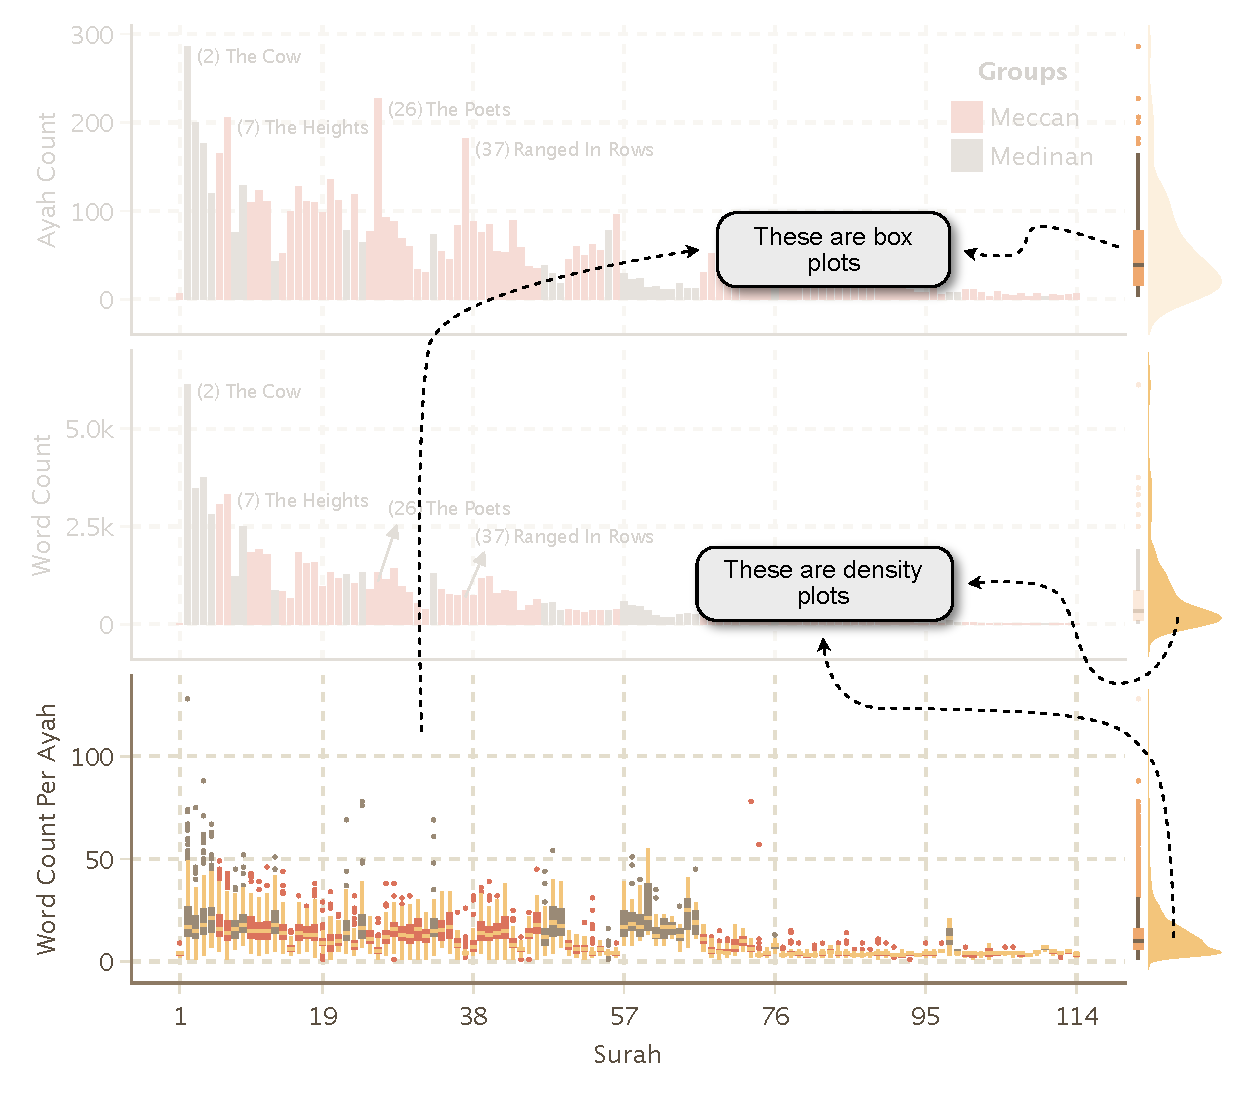
\includegraphics[width=\textwidth]{img/plot1-desc.pdf}
    \caption{Statistics of the words and \arb[trans]{ayAt} \arb{ayAt} (verses) of the Qur'\=an}
    \label{fig:ayah_word_count_with_desc}
\end{figure}

As shown in Figure \ref{fig:ayah_word_count_with_desc}, both the Box and Density plots are tied to each other. This is indeed the case because both are describing the same information but presented in different style of visualization. In fact, Histogram is also used to describe the same information as the Box and Density, and the three are therefore related. So much so, that the three can be put into one graph. As to how to interpret these, readers are referred to for further details \textcolor{red}{[to add reference]}.
\section{Topic Modeling}\label{sec:topic_modeling_method}
As presented in Chapter \ref{ch:introduction}, the first objective is to extract the thematic themes of \textit{s\=urahs} \arb{sUr} with at least 1000 words. In Statistics and Machine Learning, this task is called Topic Modeling. There are several ways to do this, but the popular methodology is to use the Latent Dirichlet Allocation (LDA) discussed in the next section.
\subsection{Latent Dirichlet Allocation}\label{sec:lda}
Latent Dirichlet Allocation (LDA) is a Statistical methodology that is based on Bayesian inference \cite{bayes,laplace1986}. It is a generative probabilisitic model for collection of discrete data such as text corpora \cite{blei2003latent}. The idea of behind this methodology is to 
\section{Large Language Models}\label{sec:llm_method}
Generative Artificial Intelligence or GenAI for short has been making waves on its effectiveness to generate texts, images, audio, video, etc. It has elevated humanity to a new level of capability. However, behind this amazing capabilities is that GenAI is by design a mathematical formula that are called \textit{model}. There are several types of \textit{models}, and one of those is the Large Language Model (LLM). The following section will discuss what LLM is and its mathematical formulation.
\subsection{Retrieval-Augmented Generation}
The problem with LLM is that it was only trained on huge but limited data, and is therefore not able to infer what should be the context when asked.
\section{Julia Code Setup}\label{sec:code_setup}
This section will discuss the coding setup
\section{Web Application using SvelteKit and Julia}
